%!TEX root = thesis.tex

\chapter{Exploratory Field Study}
\label{chap:exploratory-field-study}

\begin{chapquote}{Peter Lee, \textit{Head of Microsoft Research}, July 2014}
``If you look around at the world and where technological surprises are happening, one place is in the art world — artists who are using tech to create new experiences.''
\end{chapquote}
% http://seattletimes.com/html/businesstechnology/2024031882_microsoftresearchxml.html
% Move this quote to the start of the whole thesis.

\begin{figure}
\centering
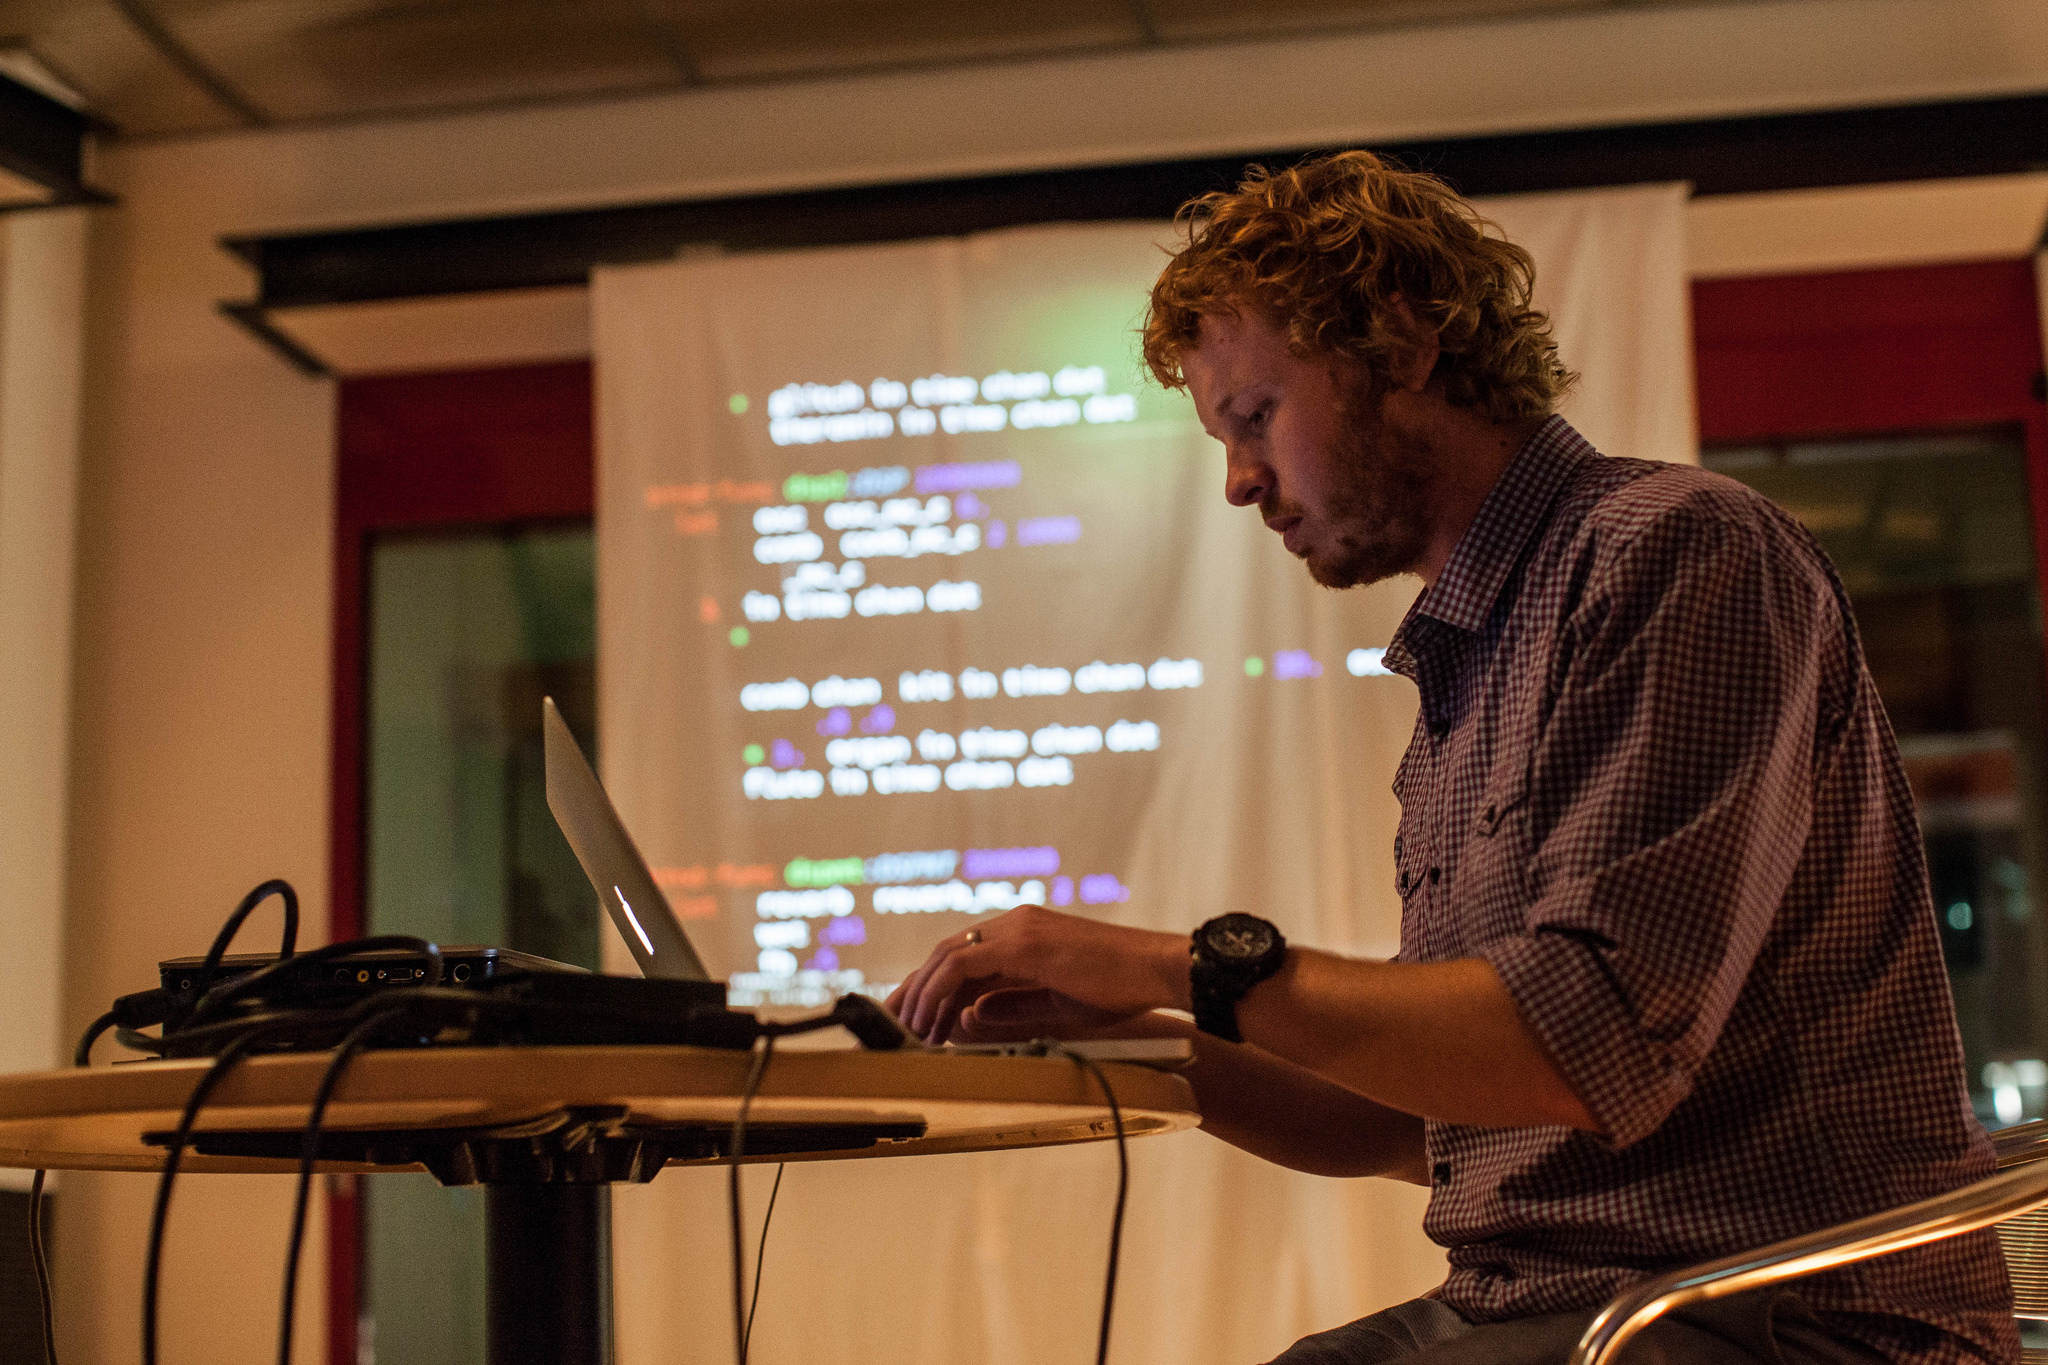
\includegraphics[width=0.9\textwidth]{../images/study-1-you-are-here-ben.jpg}
\caption{A live coder performs at the ``You Are Here'' arts festival in Canberra. An exploratory user study was conducted following the performance to examine audience perception of live coding.}
\label{fig:exploratory-field-study-ben}
\end{figure}

In order to determine a strategy for visualising source code an exploratory field study was conducted at the ``You Are Here'' arts festival in Canberra.
% Link this study to the literature review. Discuss the plan for the exploratory field study...

\section{Rationale}

The purpose of this interview was to gain insight into the audience's current understanding and enjoyment of the live coding process. Additionally, the relationship between enjoyment and understanding was to be examined. It was hoped that the examination of these factors would further inform the development of visualisations targeted at similar audiences.

\section{Method}

Audience members were asked to fill out a survey regarding their perception of and response to the projection of the computer code during the
performance. Each audience member was asked to indicate which of a
number of curves or trajectories best represented their \emph{enjoyment}
and \emph{understanding} of the performer's actions in typing the code
through the performance. These trajectories allowed for ``high'',
``medium'', and ``low'' levels of enjoyment and understanding for the
self-determined ``beginning'', ``middle'' and ``end'' of the
performance. Other survey questions addressed their sense of
``liveness'' of the performance (c.f.~\cite{Auslander}) and whether
the projected code was confusing.

\section{Participants}

A total of thirteen survey responses were received. Of these, 77\% regularly listen to music and 54\% perform regularly. 38\% of the respondents have high exposure to programming through work, study or their hobbies, as opposed to 31\% who have no experience with it. Of the respondents, 69\% had never been to a live coding performance before.

\section{Results}

Of the thirteen survey responses received, six audience members showed
a high level of enjoyment throughout the whole performance, while the
remaining seven responses showed alternating levels of enjoyment. No
audience members indicated a low level of enjoyment throughout the
performance.

Only two of the thirteen respondents indicated that they understood
the relationship between the code projections and the music throughout
the performance. Three of the six respondents who reported a high
level of enjoyment throughout the performance also indicated an
increase in understanding (from low to high) as the performance
progressed, although a Chi-square analysis revealed no significant
relationship between enjoyment and understanding due to the small
sample size. Nine of the thirteen respondents stated that the code
projection provided a sense of liveness to the performance and the
remainder stated that viewing the code had no effect on their sense of
liveness. Four respondents felt that the code projections were
confusing, five felt that they were not confusing, and four did not
answer the question.

-more comprehensive results here + graphs

% Similarly, understanding was measured according to the relative change in understanding through the performance from the beginning to the end. 31\% of survey respondents had no change to understanding through the performance. Overall, understanding is spread out more than enjoyment with only 15\% suggesting that they could understand the relationship between the visuals and the music throughout the performance. There is no statistically significant relationship ($p > .05$) between music listening habits and understanding nor is there a statistically significant relationship ($p > .05$) between coding experience and understanding.

% The relationship between enjoyment and understanding can be seen in Figure 1. Notably, three respondents who had high enjoyment throughout the performance were the only respondents who had a pattern of low to high understanding. However, the relationship between enjoyment and understanding is not statistically significant ($p > .05$).


\section{Discussion}

Taken as a whole, the results of this small field study were
salutatory towards the benefit of ``seeing as well as hearing'' code
during a live coding performance, especially as far as the general
public is concerned. The majority of the audience felt that they made
the performance seem more ``live''. However, a minority stated that
they found the projections confusing and only a very small number of
respondents claimed to have actually understood what the programmer
was doing. We were quite intrigued by the small cohort of respondents
whose understanding increased through the performance and whose
enjoyment remained high, and we wished to test whether augmenting code
projections with additional visualisations might increase the
understanding and enjoyment of the audience in live coding.

-more comprehensive discussion here
